% !TeX program = xelatex
% !TeX encoding = UTF-8
% !TeX root = verkhoturov.tex

% Command to compile document
% xelatex -synctex=1 -interaction=nonstopmode verkhoturov.tex

% Document class repo 
% https://github.com/ValeryVerkhoturov/mirea-kb2-programming-languages

\documentclass{mirea}

\usepackage{array}
\usepackage{longtable}
\usepackage{float}


\usepackage{hyperref}
\hypersetup{pdftitle={Курсовая работа 7 семестр Организация обработки больших данных}}

\newcommand{\studentname}{В.\,C.\,Верхотуров}

\usepackage{graphicx}

\usepackage{listings}
\usepackage{xcolor}
\lstset{extendedchars=\true, basicstyle=\footnotesize, breaklines=true, numbers=left, captionpos=t, showstringspaces=false, commentstyle=\color{teal}, stringstyle=\color{red}, keywordstyle=\color{violet}}  % Настройки, применяемые ко всем листингам

\usepackage{caption}
\captionsetup[lstlisting]{justification=raggedright, singlelinecheck=false}


\begin{document}
	
	\begin{titlepage}
	
	\pagestyle{empty}
	\setlength\parindent{0pt}
	\newcommand{\blankDate}[2]{\mbox{\uline{<<\makebox[.7cm]{#1}>>~\makebox[2cm]{#2}~\the\year{}~г.}}} % {день}{месяц}
	\newcommand\blankLine[2]{$\underset{\text{#1}}{\text{\uline{#2}}}$}
	\begin{center}
		\includegraphics[width=2.5cm]{MIREA_Gerb_Black} \par
		МИНОБРНАУКИ РОССИИ \par 
		Федеральное государственное бюджетное образовательное учреждение высшего образования \par
		\textbf{<<МИРЭА~--- Российский технологический университет>>} \par
		\textbf{\fontsize{16pt}{16pt}\selectfont РТУ МИРЭА} \par
		\blankLine{(наименование института, филиала)}{Институт кибербезопасности и цифровых технологий} \par
		\blankLine{(наименование кафедры)}{Кафедра КБ-14 <<Цифровые технологии обработки данных>>} \par
		\vspace*{1cm}
		{\fontsize{16pt}{16pt}\selectfont
			\textbf{КУРСОВОЙ ПРОЕКТ (РАБОТА)}} \par
		по дисциплине \blankLine{(наименование дисциплины)}{Организация обработки больших данных}
	\end{center}
	\textbf{Тема курсовой работы \uline{Организация обработки больших данных средствами Apache Spark}} \bigskip\par
	Студент группы \blankLine{учебная группа, фамилия, имя, отчество студента}{БСБО-05-20 \studentname} \hfill\blankLine{подпись студента}{\hspace{4cm}} \bigskip\par
	Руководитель курсовой работы \blankLine{}{\hspace*{4cm}} \hfill\blankLine{подпись руководителя}{\hspace{4cm}} \bigskip\par
	Член комиссии \blankLine{}{\hspace*{4cm}} \hfill\blankLine{подпись члена комиссии}{\hspace{4cm}} \bigskip\par
	\begin{tabular}{@{}ll}
		Работа предоставлена к защите & \blankDate{}{} \bigskip\\
		Допущен к защите & \blankDate{}{}
	\end{tabular}
	\begin{center}
		\vfill Москва~--- \the\year{}~г.
	\end{center}
	
	\newpage
	\begin{center}
		\includegraphics[width=2.5cm]{MIREA_Gerb_Black} \par
		МИНОБРНАУКИ РОССИИ \par 
		Федеральное государственное бюджетное образовательное учреждение высшего образования \par
		\textbf{<<МИРЭА~--- Российский технологический университет>>} \par
	\end{center}
	
	Институт ИКЦТ направление 09.03.02 <<Информационные системы и технологии>>
	
	Кафедра КБ-14 <<Цифровые технологии обработки данных>>
	
	Дисциплина <<Организация обработки больших данных>>
	
	\begin{center}
		\vspace*{1cm}
		{\fontsize{16pt}{16pt}\selectfont
			\textbf{ПОЯСНИТЕЛЬНАЯ ЗАПИСКА \\ к курсовой работе (проекту) }} \par
	\end{center}
	
	Студент \underline{\studentname} \par\vspace*{.3cm}
	Группа \underline{БСБО-05-20} \par\vspace*{.3cm}
	Работа защищена на оценку \underline{\hspace*{4cm}} \par\vspace*{.3cm}
	Руководитель работы	\underline{\hspace*{4cm}} \par\vspace*{.3cm}
	Член комиссии \underline{\hspace*{4cm}}
	\begin{center}
		\vfill Москва~--- \the\year{}~г.
	\end{center}
	
	\newpage
	\begin{center}
		\includegraphics[width=2.5cm]{MIREA_Gerb_Black} \par
		МИНОБРНАУКИ РОССИИ \par 
		Федеральное государственное бюджетное образовательное учреждение высшего образования \par
		\textbf{<<МИРЭА~--- Российский технологический университет>>} \par
	\end{center}
	
	Институт ИКЦТ направление 09.03.02 <<Информационные системы и технологии>>
	
	Кафедра КБ-14 <<Цифровые технологии обработки данных>>
	
	Дисциплина <<Организация обработки больших данных>>
	
	\begin{center}
		\vspace*{1cm}
		{\fontsize{16pt}{16pt}\selectfont
			\textbf{ЗАДАНИЕ НА КУРСОВУЮ РАБОТУ}} \par
	\end{center}
	
	Студент 4 курса группы БСБО-05-20.
	
	\begin{enumerate}
		\item Тема: Проектирование баз данных
		\item Срок представления проекта (работы) к защите:
		\item Содержание пояснительной записки:
		\begin{itemize}
			\item Содержание
			\item Краткие теоретические сведения
			\item Задание на курсовую работу
			\item Анализ социальной акивности средствами Apache Spark
			\item Заключение
			\item Литература
		\end{itemize}
	\end{enumerate}
	
	Руководитель работы \underline{\hspace*{3cm}}
	
	Задание принял к исполнению \underline{\studentname}
	
	\begin{center}
		\vfill Москва~--- \the\year{}~г.
	\end{center}
\end{titlepage}
\addtocounter{page}{3}


\tableofcontents

\section{Краткие теоретические сведения}

Resilent Distributed DataSet~\cite{bib:rdd1, bib:rdd2, bib:rdd3} --- это неизменяемая распределенная коллекция наборов данных, разделенных по множеству узлов кластера, которую можно восстановить в случае потери раздела, что обеспечивает отказоустойчивость. Он также обеспечивает встроенные вычисления в памяти и ссылается на наборы данных, хранящиеся во внешних системах хранения.

Spark SQL~\cite{bib:sql1, bib:sql2, bib:sql3} — это модуль Spark для обработки структурированных данных. Он предоставляет абстракцию программирования, называемую DataFrames, а также может действовать как механизм распределенных запросов SQL. Это позволяет немодифицированным запросам Hadoop Hive выполняться до 100 раз быстрее для существующих развертываний и данных.

GraphFrames~\cite{bib:gf1, bib:gf2, bib:gf3, bib:gf4} — это пакет для Apache Spark, который предоставляет графики на основе DataFrame. Он предоставляет API-интерфейсы высокого уровня на Scala, Java и Python. Он призван обеспечить как функциональность GraphX, так и расширенную функциональность с использованием Spark DataFrames. Эта расширенная функциональность включает в себя поиск мотивов, сериализацию на основе DataFrame и высоковыразительные графовые запросы.


\section{Задание на курсовую работу}

Часть 1. RDD, SparkSQL

Загрузить набор данных из twitter и найти пользователя из РФ, чаще остальных упоминающего фамилии российских политических деятелей (на русском).

Решить задачу необходимо средствами RDD transformations + actions и DataFrame + SparkSQL. Продемонстрировать, что ответ совпадает.

Часть 2. GraphFrames

Загрузить набор данных из twitter и найти наибольшую компоненту связности социального графа (группу пользователей, которые общаются преимущественно друг с другом) для российских пользователей.

Решить задачу необходимо средствами GraphFrames.

twitterid — идентификационный номер твита

userid — идентификационный номер пользователя (анонимизированный для пользователей, у которых на момент приостановки было менее 5000 подписчиков)

user\_display\_name — имя пользователя (закодированное как userid для анонимных пользователей)

user\_screen\_name — дескриптор пользователя в Твиттере (закодированный как идентификатор пользователя для анонимных пользователей)

user\_reported\_location — местоположение пользователя, сообщенное самим пользователем

user\_profile\_description — описание профиля пользователя

user\_profile\_url — URL профиля пользователя

follower\_count — количество аккаунтов, подписавшихся на пользователя

follow\_count — количество аккаунтов, на которые подписан пользователь

account\_creation\_date — дата создания учетной записи пользователя

account\_language — язык аккаунта, выбранный пользователем.

twitter\_language — язык твита

twitter\_text — текст твита (упоминания анонимизированных аккаунтов заменены анонимизированными идентификаторами пользователей)

twitter\_time — время публикации твита (UTC)

twitter\_client\_name — имя клиентского приложения, используемого для публикации твита.

in\_reply\_to\_tweetid — идентификатор исходного твита, на который этот твит является ответом (только для ответов)

in\_reply\_to\_userid — идентификатор пользователя исходного твита, на который этот твит является ответом (только для ответов)

quoted\_tweet\_tweetid — идентификатор исходного твита, который цитируется в этом твите (только для кавычек)

is\_retweet — True/False, является ли этот твит ретвитом

retweet\_userid — для ретвитов идентификатор пользователя, автора исходного твита.

retweet\_tweetid — для ретвитов твитид исходного твита.

latitude - географическая широта, если доступна.

longitude - долгота с географической привязкой, если доступна

quote\_count — количество твитов, цитирующих этот твит

reply\_count - количество твитов, ответивших на этот твит

like\_count — количество лайков, полученных этим твитом

retweet\_count — количество ретвитов, полученных этим твитом

hashtags — список хэштегов, использованных в этом твите.

URL-адреса — список URL-адресов, использованных в этом твите.

user\_mentions — список идентификаторов пользователей, упомянутых в этом твите (включая анонимные идентификаторы пользователей)

poll\_choices — если твит содержал опрос, в этом поле отображаются варианты опроса, разделенные знаком «|».



\section{Анализ социальной активности средствами Apache Spark}

\subsection{Анализ данных средствами RDD и SparkSQL}

Найти наибольшую компоненту связности социального графа (группу пользователей, которые общаются преимущественно друг с другом) для российских пользователей.

\begin{figure}[htb]
	\centering
	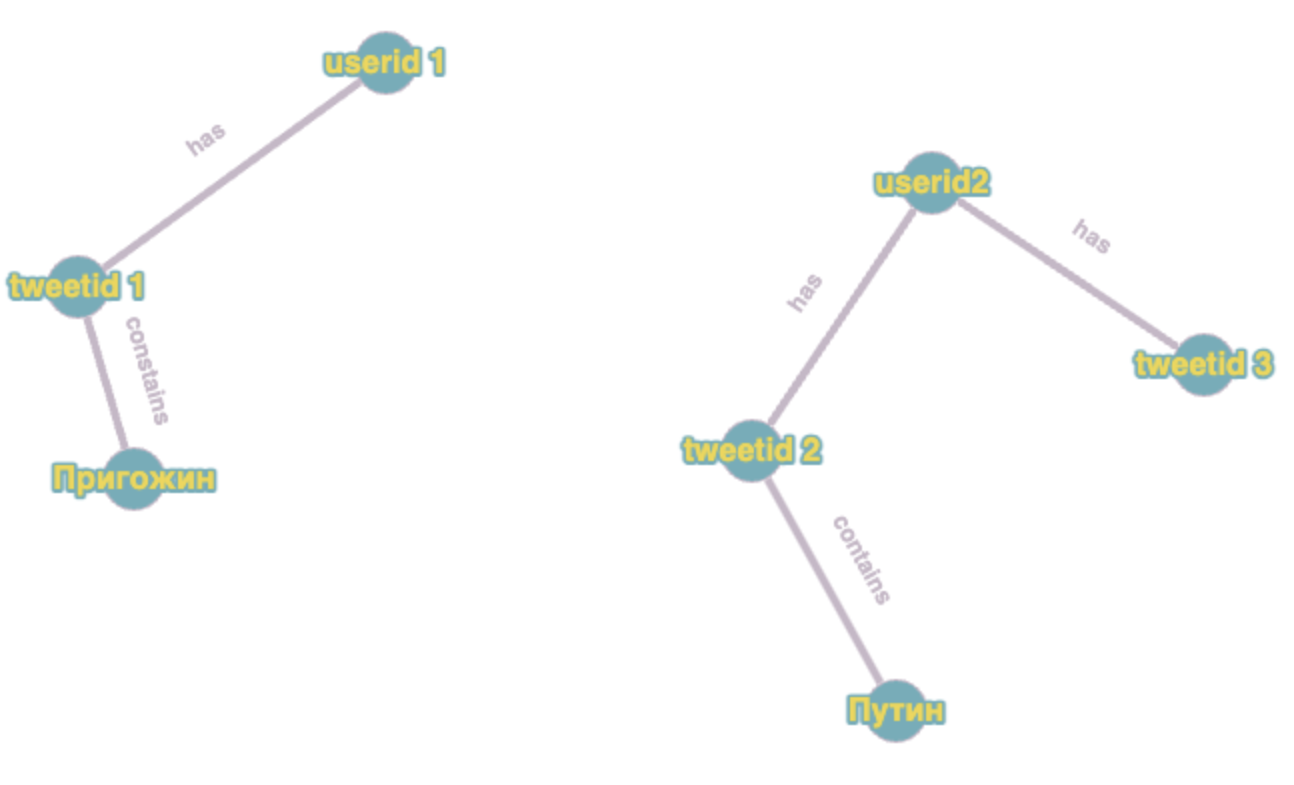
\includegraphics[width=.9\textwidth]{rddgraph.png}
	\parskip=6pt
	\caption{Визуализация датасета}
	\label{fig:gfpic}
\end{figure}

Загрузка датасета в SparkRDD:

\begin{lstlisting}[language={Python}, caption={Нахождение наибольшей компоненты связанности}, label=lst:rdd1]
def set_tweets(self, path):
	sc = SparkContext().getOrCreate()
	self.tweets = sc.textFile(path)\
		.map(lambda line: line[1:-1].split('","'))
	self.tweets = self.tweets.map(
		lambda element: 
			(element[1], 
			 element[10], 
			 element[12])
	)
\end{lstlisting}

Выбор сообщений на русском языке:

\begin{lstlisting}[language={Python}, caption={Выбор сообщений}, label=lst:rdd2]
@staticmethod
def filter_func(row):
	if row[1] == 'ru':
		for politician in politicians:
			if politician in row[2]:
				return True
	return False
	
def filter_tweets(self):
	self.tweets = self.tweets.filter(
		SparkRDD.filter_func
	)
	self.tweets = self.tweets.map(
		lambda element: 
			(element[0], str(element[2]))
	)
\end{lstlisting}

Получение userid, который чаще остальных упоминающего фамилии российских политических деятелей (на русском):

\begin{lstlisting}[language={Python}, caption={Получение userid}, label=lst:rdd3]
def get_userid(self):
	self.users_tweets = self.tweets.groupByKey()\
		.mapValues(len)
	self.sorted_tweets = self.users_tweets.sortBy(
		lambda element: element[1], ascending=False
	)
	return self.sorted_tweets.max(
		lambda element: element[1]
	)[0]
\end{lstlisting}

Указание пути и запуск SparkRDD:

\begin{lstlisting}[language={Python}, caption={Получение userid}, label=lst:rdd4]
if __name__ == '__main__':
file_path = 'hdfs:///ira_tweets_csv_hashed.csv'
sparkRDD = SparkRDD()
sparkRDD.set_tweets(file_path)
sparkRDD.filter_tweets()
print("USER_ID: " + sparkRDD.get_userid())
\end{lstlisting}

Загрузка датасета:

\begin{lstlisting}[language={Python}, caption={Получение userid}, label=lst:sql1]
self.tweets = self.spark.read.csv(path, header=True)
self.tweets.createOrReplaceTempView("tweets")
\end{lstlisting}

Создание вью, которое отдает русские сообщения:

\begin{lstlisting}[language={Python}, caption={Получение вью с русскими сообщениями}, label=lst:sql2]
def tweets_temp(self):
	query = """\
		CREATE OR REPLACE TEMP VIEW tweets_temp AS
		SELECT tweetid, 
			userid, 
			tweet_text, 
			account_language
		FROM tweets 
		WHERE account_language == 'ru' 
			and tweet_language == 'ru'
	"""
	self.spark.sql(query)
\end{lstlisting}

Получение userid, который чаще остальных упоминающего фамилии российских политических деятелей (на русском):

\begin{lstlisting}[language={Python}, caption={Получение userid}, label=lst:sql3]
def get_userid(self):
	query = f"SELECT userid FROM tweets_temp " +\
		"WHERE tweet_text " +\
		"LIKE '%{self.politicians[0]}%'"
	for politician in self.politicians[1:]:
		query += f" OR tweet_text '" +\
		f"LIKE '%{politician}%'"
		query += f" GROUP BY userid " +\
			"ORDER BY COUNT(tweetid) DESC LIMIT 1"
		return self.spark.sql(query).show()
\end{lstlisting}

Указание пути и запуск SparkSQL:

\begin{lstlisting}[language={Python}, caption={Запуск SparkSQL}, label=lst:sql4]
if __name__ == '__main__':
	file_path = 'hdfs:///ira_tweets_csv_hashed.csv'
	sparkSQL = SparkSQL()
	sparkSQL.set_tweets(file_path)
	sparkSQL.tweets_temp()
	print(sparkSQL.get_userid())
\end{lstlisting}

\subsection{Анализ данных средствами GraphFrames}

Найти наибольшую компоненту связности социального графа (группу пользователей, которые общаются преимущественно друг с другом) для российских пользователей.

\begin{figure}[htb]
	\centering
	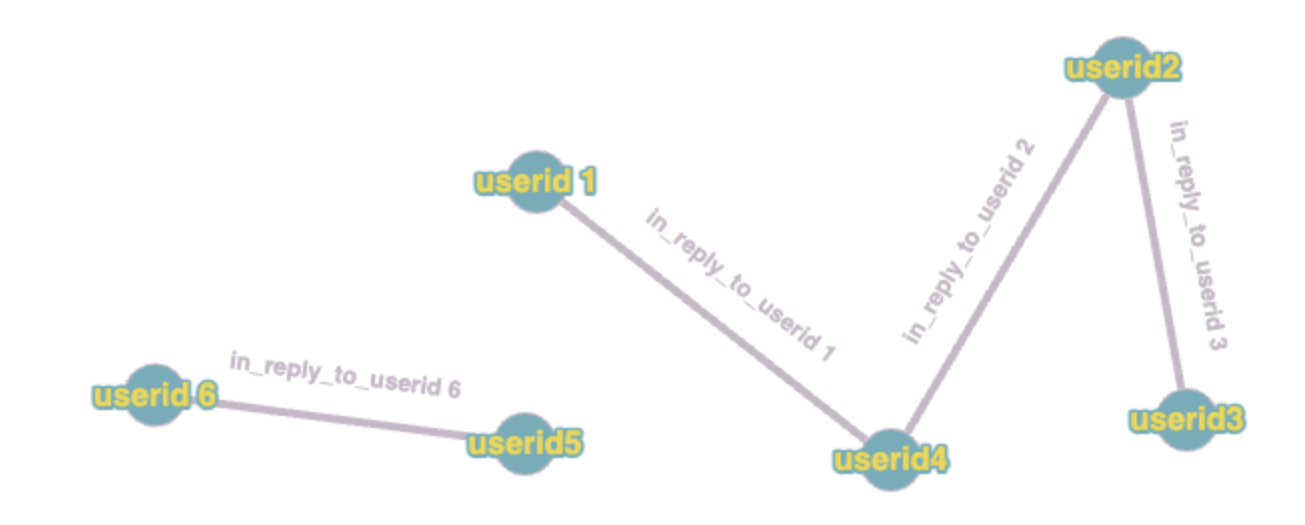
\includegraphics[width=.9\textwidth]{graph.png}
	\parskip=6pt
	\caption{Визуализация создаваемого графа}
	\label{fig:gfpic}
\end{figure}

Создание графа с пользователями в вершине:

\begin{lstlisting}[language={Python}, caption={Создание графа}, label=lst:gf1]
def set_graphframe(self, path):
	self.tweets = self.spark\
		.read.csv(path, header=True)
	self.tweets.createGlobalTempView("users")
	self.filtered_users = self.spark.sql(
		"SELECT * FROM global_temp.users " +\
		"WHERE user_reported_location " +\
		"LIKE '%" +\
			"Россия" +\
			"%'"
	)
	vertices = self.filtered_users\
		.select('userid').toDF('id')
	edges = self.filtered_users\
		.select('userid', 'in_reply_to_userid')\
		.toDF('src', 'dst')
	edges = edges.filter(edges.dst != 'null')
	self.gf = GraphFrame(vertices, edges)
\end{lstlisting}

Получение связанных компонент:

\begin{lstlisting}[language={Python}, caption={Получение связанных компонент}, label=lst:gf2]
def get_components(self):
	components = self.gf.connectedComponents()
	components.createOrReplaceTempView("components")
\end{lstlisting}

Получение наибольшей компоненты связности:

\begin{lstlisting}[language={Python}, caption={Получение наибольшей компоненты связанности}, label=lst:gf3]
def get_max_component(self):
	self.get_components()
	query = """
		SELECT component, COUNT(*) 
		AS count 
		FROM components
		GROUP BY component 
		ORDER BY count 
		DESC 
	"""
	return self.spark.sql(query).show()
\end{lstlisting}


\section*{Заключение}
\phantomsection
\addcontentsline{toc}{section}{Заключение}

В ходе выполнения первой задачи была допущена погрешность~--- для поиска политиков использовался заранее заданный список фамилий, в который могли войти не все политики России, упоминающиеся в датасете. 

При выполнении второй практической иногда невозможно было определить местоположение пользователя, т.к. не было заполнено поле \newline user\_reported\_location.


\begin{thebibliography}{99\kern\bibindent}
	\bibitem{bib:rdd1} Zaharia, Matei, et al. "Resilient distributed datasets: A {Fault-Tolerant} abstraction for {In-Memory} cluster computing." 9th USENIX Symposium on Networked Systems Design and Implementation (NSDI 12). 2012.
	
	\bibitem{bib:rdd2} Zaharia, Matei, et al. "Resilient distributed datasets." A fault-tolerant abstraction for in-memory cluster computing in Proceedings of the 9th USENIX conference on Networked Systems Design and Implementation. 2014.
	
	\bibitem{bib:rdd3} Deng, Changshou, et al. "A parallel version of differential evolution based on resilient distributed datasets model." Bio-Inspired Computing--Theories and Applications: 10th International Conference, BIC-TA 2015 Hefei, China, September 25-28, 2015, Proceedings 10. Springer Berlin Heidelberg, 2015.
	
	\bibitem{bib:sql1} Armbrust, Michael, et al. "Spark sql: Relational data processing in spark." Proceedings of the 2015 ACM SIGMOD international conference on management of data. 2015.
	
	\bibitem{bib:sql2} Baldacci, Lorenzo, and Matteo Golfarelli. "A cost model for SPARK SQL." IEEE Transactions on Knowledge and Data Engineering 31.5 (2018): 819-832.
	
	\bibitem{bib:sql3} Ivanov, Todor, and Max-Georg Beer. "Evaluating hive and spark SQL with BigBench." arXiv preprint arXiv:1512.08417 (2015).
	
	\bibitem{bib:gf1} Dave, Ankur, et al. "Graphframes: an integrated api for mixing graph and relational queries." Proceedings of the fourth international workshop on graph data management experiences and systems. 2016.
	
	\bibitem{bib:gf2} Mishra, Raju Kumar, et al. "GraphFrames." PySpark SQL Recipes: With HiveQL, Dataframe and Graphframes (2019): 297-315.
	
	\bibitem{bib:gf3} Bahrami, Ramazan Ali, Jayati Gulati, and Muhammad Abulaish. "Efficient processing of SPARQL queries over graphframes." Proceedings of the International Conference on Web Intelligence. 2017.
	
	\bibitem{bib:gf4} Popov, Alexander, and Jennifer Sikos. "Graph embeddings for frame identification." Proceedings of the International Conference on Recent Advances in Natural Language Processing (RANLP 2019). 2019.
	
\end{thebibliography}
	
\end{document}
